\documentclass[conference,a4paper]{IEEEtran}

\usepackage[T2A,T1]{fontenc}
\usepackage[utf8]{inputenc}
\usepackage[english,bulgarian]{babel}
\usepackage{tempora}
\usepackage{newtxmath}
\usepackage{microtype}
\usepackage{amsmath}
\usepackage{graphicx}
\usepackage{float}
\usepackage{booktabs}
\usepackage{xcolor}
\usepackage{tikz}
\usetikzlibrary{positioning,arrows.meta,fit,calc}
\usepackage{fontawesome5}
\usepackage{pgfplots}
\pgfplotsset{compat=1.18}
\usepackage[autostyle]{csquotes}
\DeclareQuoteStyle{bulgarian}{\quotedblbase}{\textquotedblleft}{\quotesinglbase}{\textquoteleft}
\usepackage{url}
\usepackage[hidelinks]{hyperref}
\usepackage[nameinlink]{cleveref}
\crefname{figure}{фиг.}{фиг.}
\Crefname{figure}{Фигура}{Фигури}
\crefname{table}{табл.}{табл.}
\Crefname{table}{Таблица}{Таблици}
\crefname{equation}{формула}{формули}
\Crefname{equation}{Формула}{Формули}
\crefname{section}{раздел}{раздели}
\Crefname{section}{Раздел}{Раздели}
\newcommand{\crefrangeconjunction}{--}
\newcommand{\crefpairconjunction}{ и }
\newcommand{\crefmiddleconjunction}{, }
\newcommand{\creflastconjunction}{ и }

\addto\captionsbulgarian{%
  \renewcommand{\figurename}{Фигура}%
  \renewcommand{\tablename}{Таблица}%
  \renewcommand{\abstractname}{Резюме}%
  \renewcommand{\refname}{\bgsc{И}{зползвана литература}}}
\renewcommand{\IEEEkeywordsname}{Ключови думи}

% Let more floats share a page with text.
\renewcommand{\topfraction}{0.9}
\renewcommand{\dbltopfraction}{0.9}
\renewcommand{\textfraction}{0.1}
\renewcommand{\floatpagefraction}{0.8}
\renewcommand{\dblfloatpagefraction}{0.8}
\setcounter{topnumber}{3}
\setcounter{dbltopnumber}{2}

\graphicspath{{figures/}{../figures/}}

% Tempora has no Cyrillic small caps: imitate them for section headings.
% Usage: \bgsc{first letter}{rest of the heading}
\newcommand{\bgsc}[2]{\texorpdfstring{#1{\footnotesize\MakeUppercase{#2}}}{#1#2}}
\newcommand{\Ffeat}{\mathbf{F}}
\newcommand{\film}{\mathrm{FiLM}}
\newcommand{\code}[1]{\textlatin{\texttt{#1}}}
\newcommand{\en}[1]{\enquote{#1}}

\begin{document}

\title{Сегментиране на обекти по текстово описание\\чрез замразени CLIP признаци и пренасяне в 3D}

\author{\IEEEauthorblockN{Асен Попов}
\IEEEauthorblockA{\textit{Факултет по компютърни системи и технологии}\\
\textit{Технически университет -- София}\\
София, България\\
\textlatin{asepopov@tu-sofia.bg}}}

\maketitle

\begin{abstract}
Робот, на когото е казано \en{pick up the cup on the left}, трябва първо да намери пикселите, а след
това и 3D точките, към които се отнася изречението. В настоящата работа се изследва доколко малък
обучаем декодер върху \emph{замразен} CLIP енкодер може да реши тази задача за сегментиране по
референтен израз. Получените маски се пренасят в облак от точки в световна координатна система чрез
калибрирана RGB-D камера. Обучава се само декодерът: 1.05\,M параметъра, или 0.7\% от 151\,M
параметъра на целия модел, докато CLIP енкодерите със 150\,M параметъра остават замразени и
признаците им се изчисляват еднократно. При обучение с по-малко от 4\,000 изречения обуславянето по
текст чрез FiLM повишава mIoU върху тестовото множество от 0.281 (само изображение) до 0.393,
наравно с CLIPSeg (0.385), който използва същия замразен CLIP и декодер с подобен размер, обучен
върху много по-голям набор от данни. Двата модела имат допълващи се силни страни:
предложеният декодер е по-добър при пространствени указания, а CLIPSeg при имена на обекти и
атрибути.
\end{abstract}

\begin{IEEEkeywords}
CLIP, FiLM, RGB-D обратна проекция, облаци от точки, сегментиране по референтен израз
\end{IEEEkeywords}

% ---------------------------------------------------------------------------
\section{\bgsc{В}{ъведение}}
\label{sec:introduction}

Роботите в домовете и складовете все по-често получават инструкции на естествен език. Преди
манипулаторът да може да действа спрямо \en{the white armchair} или \en{the woman in the middle},
системата за възприятие трябва да отговори на два геометрични въпроса: \emph{кои пиксели} описва
изречението и \emph{къде в пространството} се намират те. Първият въпрос е задачата за сегментиране
по референтен израз (referring image segmentation) \cite{hu2016segmentation}. Вторият е класическа
задача от компютърната графика и компютърното зрение: обръщане на проекцията на камерата с помощта
на измерена дълбочина \cite{hartley2004mvg}.

Големите модели за зрение и език, като CLIP \cite{radford2021clip}, правят първия въпрос значително
по-достъпен: техните представяния на изображения и текст са в общо пространство и се пренасят към
много задачи без преобучение. Пълното им дообучение обаче е скъпо и лесно води до преобучение
(overfitting) при малки набори от данни. Оттук произтича изследваният в тази работа въпрос:
\emph{може ли лек декодер, обучен върху замразени CLIP признаци от малък набор от данни, да свързва
референтни изрази с обекти достатъчно добре, за да локализира търсения обект в 3D?}

Приносите на работата са:
\begin{itemize}[\setlength{\IEEElabelindent}{0pt}]
\item декодер с 1.05\,M параметъра, който обединява CLIP токени на участъци от няколко слоя с
  представянето на изречението чрез признакова линейна модулация (FiLM) \cite{perez2018film};
\item контролирано сравнение на модел само по изображение, обединяване чрез FiLM и чрез
  конкатенация, на функцията на загубата и на регуляризацията, включително хоризонтално отражение,
  при което думите \en{left} и \en{right} също се разменят; всеки вариант е обучен три пъти и
  оценен върху отделено тестово множество;
\item сравнение с предварително обучения модел CLIPSeg \cite{luddecke2022clipseg}, разделено по
  тип на изречението;
\item геометричен модул, който пренася предсказаната маска от RGB-D кадри в обща световна
  координатна система, с проверка за съгласуваност между няколко гледни точки.
\end{itemize}

% ---------------------------------------------------------------------------
\section{\bgsc{П}{реглед на свързаните работи}}
\label{sec:related}

\subsection{Модели за зрение и език и плътно предсказване}

CLIP \cite{radford2021clip} обучава контрастивно енкодер за изображения, в случая Vision Transformer
(ViT) \cite{dosovitskiy2021vit}, и енкодер за текст върху 400 милиона двойки изображение--текст.
Глобалните му представяния позволяват класификация без допълнително обучение (zero-shot), но
сегментирането изисква плътен изход за всеки пиксел. MaskCLIP \cite{zhou2022maskclip} показва, че
токените на участъците във ViT носят използваема пространствена информация и без обучение, а LSeg
\cite{li2022lseg} обучава енкодер за изображения, чиито представяния на ниво пиксел съвпадат с CLIP
текстовите представяния на имена на класове. Най-близък до настоящата работа е CLIPSeg
\cite{luddecke2022clipseg}: той запазва CLIP замразен и добавя малък трансформърен декодер,
обусловен от подканата чрез FiLM \cite{perez2018film}, обучен върху набора PhraseCut
\cite{wu2020phrasecut}. Тук той служи като външна отправна точка.

\subsection{Сегментиране по референтен израз}

При сегментирането по референтен израз \cite{hu2016segmentation} се предсказва маската на единствения
обект, описан от изречението, като за това може да са нужни атрибути (\en{girl in pink}), отношения
или положение (\en{man on far left}). Стандартните набори RefCOCO и RefCOCO+
\cite{kazemzadeh2014referitgame,yu2016refcoco} са изградени върху изображения от COCO
\cite{lin2014coco}. Най-добрите модели, като CRIS \cite{wang2022cris} и LAVT \cite{yang2022lavt},
дообучават големи енкодери с кросмодално внимание върху десетки хиляди изображения. Настоящата работа
съзнателно разглежда много по-ограничен режим: замразен енкодер, декодер с около един милион
параметъра и по-малко от хиляда обучаващи изображения.

\subsection{Възприятие в 3D, обусловено от език}

В роботиката CLIPort \cite{shridhar2021cliport} съчетава семантиката на CLIP с пространствени
пътища за манипулация върху маса. OpenScene \cite{peng2023openscene}, ConceptFusion
\cite{jatavallabhula2023conceptfusion} и LERF \cite{kerr2023lerf} прикрепят CLIP признаци към 3D
облаци от точки, обединени карти или полета на излъчване, така че сцената да може да се търси с
текст. Тези системи първо изграждат пълно 3D представяне. Тук е избран по-простият и по-евтин път:
сегментирането се извършва в 2D и само избраните пиксели се пренасят в 3D чрез модела на камера
с точков отвор (pinhole) \cite{hartley2004mvg}, с помощта на Open3D \cite{zhou2018open3d}.

% ---------------------------------------------------------------------------
\section{\bgsc{Ф}{ормулировка на задачата}}
\label{sec:problem}

При дадено RGB изображение $I \in [0,255]^{H\times W\times 3}$ и референтно изречение $t$ целта е
двоична маска $M \in \{0,1\}^{H\times W}$ на обекта, описан от $t$. Моделът извежда карта на
вероятностите $P(u,v) = p(\text{обект} \mid I, t)$, която се прагува при $0.5$. За пример с
истинска маска $G$ се изчисляват
\begin{equation}
\mathrm{IoU} = \frac{|M \cap G|}{|M \cup G|}, \qquad
\mathrm{Dice} = \frac{2\,|M \cap G|}{|M| + |G|},
\label{eq:metrics}
\end{equation}
върху решетка $224\times 224$. Отчита се средното по изречения (mIoU, среден Dice) и P@0.5, делът
на изреченията с $\mathrm{IoU} > 0.5$, който може да се тълкува като \enquote{обектът е намерен}.

Ако освен това са известни картата на дълбочината $D$, вътрешните параметри на камерата $K$ и
позата на камерата $T_{wc}$, втората цел е множеството от 3D точки на обекта в световни
координати, неговият център на тежестта и обхващащата го кутия.

% ---------------------------------------------------------------------------
\section{\bgsc{М}{етод}}
\label{sec:method}

\begin{figure*}[t]
\centering
\resizebox{\textwidth}{!}{% Pipeline overview, Bulgarian labels (Figure 1). Included from main_bg.tex.
\begin{tikzpicture}[
  font=\footnotesize,
  >={Stealth[length=1.8mm]},
  arr/.style={->, thick, black!70},
  lbl/.style={font=\scriptsize, text=black!75, align=center},
  thumb/.style={inner sep=0pt, draw=black!40, line width=0.4pt}]

  % colours
  \colorlet{frozenC}{blue!55!cyan}
  \colorlet{trainC}{orange!85!red}
  \colorlet{geoC}{green!50!black}

  % encoder: trapezium narrowing to the right
  \newcommand{\encoder}[3]{% centre, name, text
    \fill[frozenC!15, draw=frozenC, line width=0.6pt, rounded corners=1.5pt]
      ($#1+(-0.65,0.75)$) -- ($#1+(0.65,0.45)$) -- ($#1+(0.65,-0.45)$) -- ($#1+(-0.65,-0.75)$) -- cycle;
    \node[lbl, text=frozenC!60!black] (#2) at #1 {#3};
    \node[text=frozenC, font=\small] at ($#1+(0,1.0)$) {\faSnowflake};}

  % ---------------- image branch ----------------
  \node[thumb, anchor=center] (rgb) at (0,0) {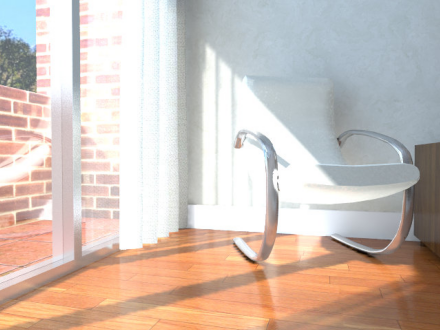
\includegraphics[width=2.1cm]{fig1_rgb.png}};
  \node[lbl, below=1mm of rgb] {RGB изображение};

  \encoder{(2.75,0)}{ienc}{Енкодер за\\изображения}

  % multi-layer patch tokens: four stacked grids
  \begin{scope}[shift={(4.55,-0.55)}]
    \foreach \k/\c in {3/frozenC!20, 2/frozenC!35, 1/frozenC!50, 0/frozenC!65} {
      \begin{scope}[shift={(0.13*\k,0.13*\k)}]
        \fill[\c, draw=frozenC!70!black, line width=0.4pt] (0,0) rectangle (0.9,0.9);
        \draw[white, line width=0.25pt, step=0.15] (0,0) grid (0.9,0.9);
      \end{scope}
    }
  \end{scope}
  \coordinate (tok) at (5.0,-0.1);
  \node[lbl] at (5.2,-0.95) {4 слоя\\$14{\times}14$ токена};

  % decoder: growing feature maps
  \foreach \s/\x/\n in {0.55/6.95/d1, 0.8/7.95/d2, 1.05/9.2/d3, 1.3/10.65/d4} {
    \node[draw=trainC!80!black, fill=trainC!25, line width=0.5pt, minimum size=\s cm,
          inner sep=0pt, rounded corners=1pt, font=\scriptsize, text=trainC!50!black] (\n) at (\x,0) {};
  }
  \draw[arr] (d1) -- (d2);
  \draw[arr] (d2) -- (d3);
  \draw[arr] (d3) -- (d4);
  \node[font=\scriptsize, text=trainC!50!black] at (d1) {$14^2$};
  \node[font=\scriptsize, text=trainC!50!black] at (d2) {$28^2$};
  \node[font=\scriptsize, text=trainC!50!black] at (d3) {$56^2$};
  \node[font=\scriptsize, text=trainC!50!black] at (d4) {$224^2$};
  \node[font=\small, text=trainC] (fire) at (8.8,1.0) {\faFire};
  \node[lbl, right=0.5mm of fire, text=trainC!70!black] {Декодер};
  \draw[trainC!60, dashed, rounded corners=3pt] (6.45,-0.95) rectangle (11.45,0.85);

  \node[thumb] (mask) at (13.1,0) {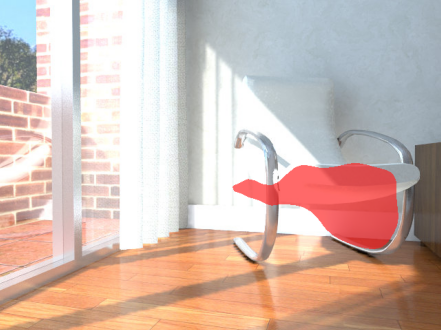
\includegraphics[width=2.1cm]{fig1_mask.png}};
  \node[lbl, below=1mm of mask] {маска $P(u,v)$};

  \node[thumb] (cloud) at (16.75,0) {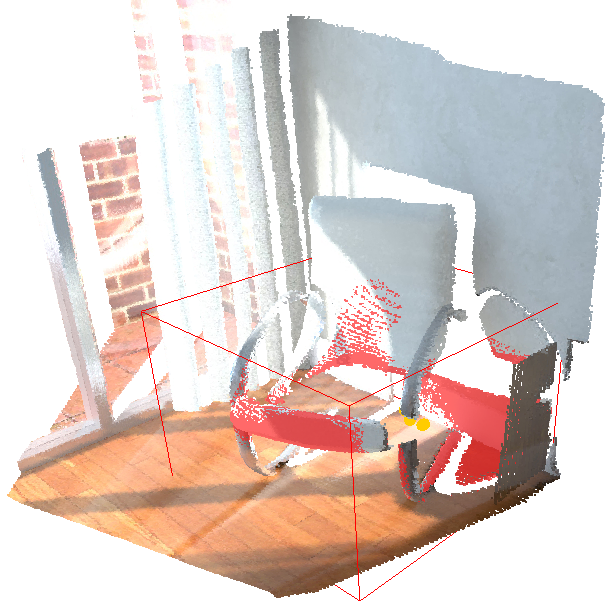
\includegraphics[width=2.0cm]{fig1_cloud.png}};
  \node[lbl, below=1mm of cloud] {3D обект в световни\\координати};

  \draw[arr] (rgb) -- (2.1,0);
  \draw[arr] (3.4,0) -- (4.5,0);
  \draw[arr] (5.95,0) -- (d1);
  \draw[arr] (d4) -- (mask);
  \draw[arr, geoC, line width=1pt] (mask.east) -- node[lbl, above, text=geoC!70!black] {към 3D} (cloud.west);

  % ---------------- text branch ----------------
  \node[draw=black!50, fill=black!4, rounded corners=6pt, inner sep=4pt, font=\small\itshape]
    (txt) at (0,-2.35) {\textlatin{\enquote{white armchair}}};
  \encoder{(2.75,-2.35)}{tenc}{Текстов\\енкодер}

  % embedding vector
  \begin{scope}[shift={(4.8,-2.35)}]
    \foreach \i in {0,...,7} \fill[frozenC!25!white!80!frozenC, draw=frozenC!70!black, line width=0.3pt]
      (-0.12,-0.6+0.15*\i) rectangle (0.12,-0.45+0.15*\i);
  \end{scope}
  \node[lbl] at (4.8,-3.15) {512-мерен};

  \node[circle, draw=trainC!80!black, fill=trainC!25, inner sep=1.5pt, lbl] (mlp) at (6.25,-2.35) {MLP};
  \node[lbl, text=trainC!70!black] at (7.55,-2.0) {$(\gamma,\beta)$};

  \draw[arr] (txt) -- (2.1,-2.35);
  \draw[arr] (3.4,-2.35) -- (4.6,-2.35);
  \draw[arr] (5.0,-2.35) -- (mlp);
  % FiLM into the first two decoder stages
  \draw[arr, trainC!80!black] (mlp.east) -| (d1.south |- 0,-1.25) -- (d1.south);
  \draw[arr, trainC!80!black] (mlp.east) -| (d2.south |- 0,-1.25) -- (d2.south);
  \node[lbl, text=trainC!70!black, anchor=west] at (8.35,-1.55) {FiLM: $(1+\gamma)\odot\Ffeat+\beta$};

  % ---------------- depth branch ----------------
  \node[thumb] (depth) at (14.9,-2.35) {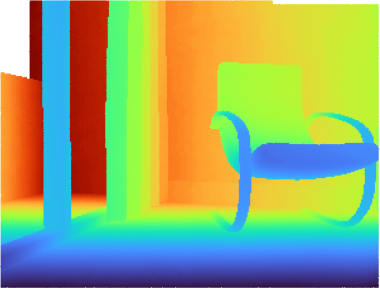
\includegraphics[width=1.7cm]{fig1_depth.png}};
  \node[lbl, right=1.5mm of depth, anchor=west] {дълбочина $D$\\$K$, $T_{wc}$};
  \draw[arr, geoC] (depth.north) -- (14.9,-0.05);
  \node[lbl, text=geoC!70!black, anchor=north] at (14.9,-3.15) {$P_w = T_{wc}\,Z K^{-1}[u,v,1]^\top$};
\end{tikzpicture}
}
\caption{Общ вид на метода. \textcolor{blue!55!cyan}{\faSnowflake}~замразени CLIP енкодери;
\textcolor{orange!85!red}{\faFire}~обучаем декодер (1.05\,M параметъра), обусловен от изречението
чрез FiLM; зелено: пренасяне на маската в 3D с калибриран RGB-D кадър.}
\label{fig:pipeline}
\end{figure*}

\Cref{fig:pipeline} показва цялата последователност от стъпки.

\subsection{Замразени CLIP признаци}

Използва се публичният модел \code{openai/clip-vit-base-patch16}. Изображение, преоразмерено до
$224\times224$, дава $14\times14$ токена на участъци с размерност 768 във всеки от 12-те
трансформърни слоя. Ранните слоеве са по-пространствени, а късните по-семантични, затова се запазват
токените от слоеве 3, 6, 9 и 12 (класовият токен се премахва). Изречението се кодира от текстовия
енкодер на CLIP в 512-мерен вектор $e_t$. Двата енкодера са замразени, така че изходите им се
изчисляват веднъж и се кешират, а едно пълно обучение отнема 30--40\,s на графичен процесор на
лаптоп.

\subsection{Декодер, обусловен от текст}

Всяка от четирите карти от токени $z_\ell$ се нормализира и проектира към $C = 128$ канала, след
което проекциите се сумират:
\begin{equation}
\Ffeat_0 = \sum_{\ell \in \{3,6,9,12\}} W_\ell \, \mathrm{LN}(z_\ell) \in \mathbb{R}^{14\times14\times C}.
\end{equation}
Текстът влиза чрез FiLM \cite{perez2018film}: малък многослоен перцептрон (MLP) преобразува $e_t$
в мащаб $\gamma$ и отместване $\beta$ за всеки канал, които модулират картата от признаци
\begin{equation}
\film(\Ffeat \mid t) = \bigl(1 + \gamma(e_t)\bigr) \odot \Ffeat + \beta(e_t).
\label{eq:film}
\end{equation}
Перцептронът се инициализира с нули, така че в началото на обучението $\gamma = \beta = 0$ и FiLM
пропуска признаците без промяна. FiLM се прилага на
два етапа: при $14\times14$ и след първото увеличаване на разделителната способност. След това
декодерът обработва признаците с конволюционни блокове $3\times3$ при $14^2$, $28^2$ и $56^2$,
предсказва по един логит за пиксел с конволюция $1\times1$ и увеличава билинейно до
$224\times224$.

За контрол се използват същият декодер \emph{без} текст (M0, само изображение) и вариант, при който
текстовият вектор се разпространява по пространството и се конкатенира към признаците вместо FiLM
(M1b, конкатенация). Тествано е и добавянето на нормализирани координатни канали $(x,y)$
\cite{liu2018coordconv}, които могат да помогнат на конволюционните мрежи с думи за положение.

\subsection{Функция на загубата и обучение}

Декодерът се обучава с двоична кръстосана ентропия (BCE) плюс мек Dice \cite{milletari2016vnet},
който компенсира дисбаланса между малки обекти и голям фон:
\begin{equation}
\mathcal{L} = \mathrm{BCE}(P, G) + \lambda \left(1 - \frac{2\sum P\,G + \epsilon}{\sum P + \sum G + \epsilon}\right),
\quad \lambda = 1.
\end{equation}
Оптимизацията използва AdamW \cite{loshchilov2019adamw} (скорост на обучение $3\cdot10^{-4}$,
тегловно затихване $0.01$), график one-cycle \cite{smith2019onecycle}, пакети от 32 примера, най-много
30 епохи и ранно спиране по mIoU върху валидационното множество.

\subsection{Хоризонтално отражение, съобразено с езика}

Хоризонталното отражение е стандартна аугментация при сегментиране, но то променя смисъла на
референтните изрази: след отражение \en{man on the left} се оказва вдясно. Затова изображението и
маската се отразяват, а думите \en{left} и \en{right} в изречението се разменят, преди то да бъде
кодирано. Размяната засяга 48\% от всички изречения в набора, така че обикновено отражение би дало
грешни етикети за почти половината обучаващи данни. Отразените CLIP признаци се кешират по същия
начин като оригиналните.

\subsection{Пренасяне на маската в 3D}
\label{sec:method-3d}

При подравнена карта на дълбочината $D$ (в милиметри) и вътрешни параметри
$K = \bigl[\begin{smallmatrix} f_x & 0 & c_x\\ 0 & f_y & c_y \\ 0 & 0 & 1\end{smallmatrix}\bigr]$
моделът на камера с точков отвор $\lambda[u,v,1]^\top = K P_c$ се обръща за всеки пиксел от
маската:
\begin{equation}
Z = \frac{D(u,v)}{1000},\quad X = \frac{(u - c_x)\,Z}{f_x},\quad Y = \frac{(v - c_y)\,Z}{f_y}.
\label{eq:backproject}
\end{equation}
Точките в координатите на камерата се пренасят в световната система чрез твърдата поза на камерата
$T_{wc} = \bigl[\begin{smallmatrix} R & \mathbf{t} \\ \mathbf{0}^\top & 1\end{smallmatrix}\bigr]$:
\begin{equation}
P_w = R\,P_c + \mathbf{t}.
\label{eq:world}
\end{equation}
Пикселите без дълбочина или по-далеч от 4\,m се пропускат. Преди пренасянето маската се изчиства в
2D: свързаните компоненти, по-малки от 10\% от най-голямата, се премахват, а маската се ерозира с 3
пиксела, защото по контура на обекта сензорът често измерва фона зад него, което би създало
\enquote{летящи} точки между обекта и стената. След пренасянето пространството се разделя на
кубчета (воксели) със страна 1\,cm и точките във всяко кубче се заменят с една средна точка, което
изравнява гъстотата на облака. Накрая се премахват изолираните точки (шум): точка, чието средно
разстояние до 20-те ѝ най-близки съседи надвишава средното за облака с повече от две стандартни
отклонения, се отстранява \cite{rusu2008objectmaps}. Обектът се описва с
центъра си на тежестта и с обхващаща кутия, успоредна на осите.

За обратната проекция, трансформацията и визуализацията се използва Open3D \cite{zhou2018open3d}.
Модулни тестове със синтетична дълбочина, $f_x \neq f_y$ и изместен главен център проверяват, че
библиотеката реализира точно \cref{eq:backproject,eq:world}, включително конвенцията на Open3D да
пази обратната поза (от свят към камера) като \enquote{външна} (extrinsic) матрица.

% ---------------------------------------------------------------------------
\section{\bgsc{Е}{кспериментална постановка}}
\label{sec:setup}

\subsection{Данни}

Данните са от RefCOCO-M \cite{refcocom}, повторно анотиране на RefCOCO \cite{yu2016refcoco} с
прецизни маски на ниво пиксел: 1\,190 изображения от COCO, 2\,080 маски на обекти и 5\,598
референтни изречения. Наборът се разпространява като едно цяло, затова е разделен \emph{по
изображения} (с фиксирано случайно разбъркване) на обучаващо, валидационно и тестово множество с 833/178/179
изображения (3\,952/857/789 изречения). Разделянето по изображения гарантира, че нито едно тестово
изображение, нито обект в него, не е виждано по време на обучението. Около две трети от
изреченията съдържат думи за положение (\en{left}, \en{right}, \en{behind}, \en{second}, \dots).

За 3D експериментите се използва примерът Redwood RGB-D, разпространяван с Open3D
\cite{choi2015redwood}: пет кадъра $640\times480$ от рендерирана всекидневна с подравнена
дълбочина, вътрешни параметри ($f_x = f_y = 525$, $c_x = 319.5$, $c_y = 239.5$) и поза на камерата
за всеки кадър.

% Wide figure defined here so that it lands on the page where it is first mentioned.
\begin{figure*}[t]
\centering
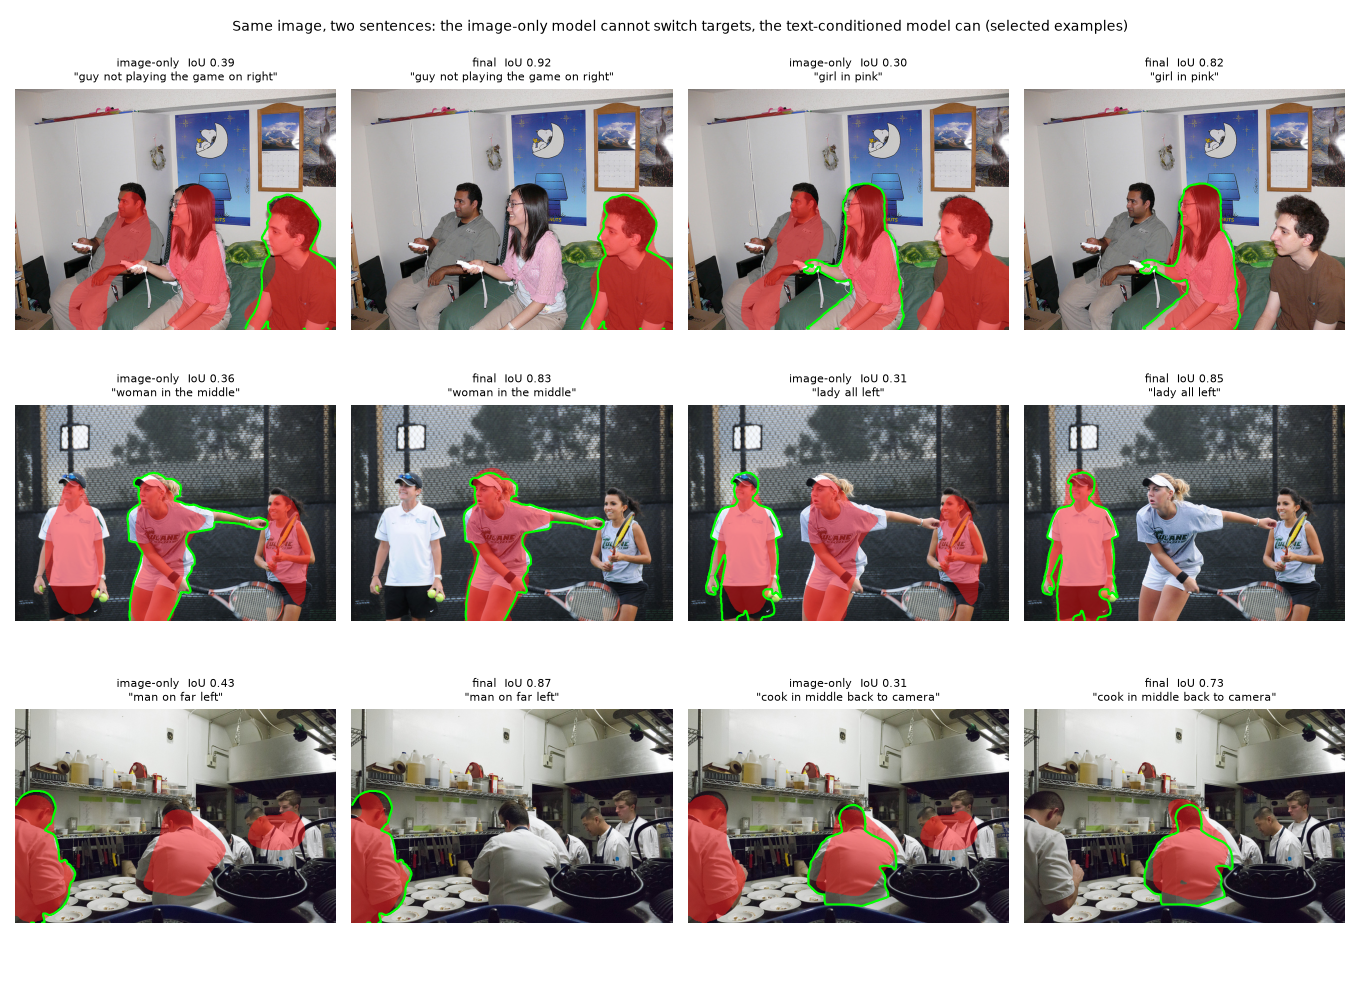
\includegraphics[width=0.92\textwidth, trim=0 228 0 40, clip]{gallery_language.png}
\caption{Едно изображение, две изречения (тестово множество). Колони 1 и 3: декодер само по
изображение (\textlatin{image-only}); колони 2 и 4: финален FiLM модел (\textlatin{final}). Зелен
контур: истинска маска; червено: предсказание. Моделът само по изображение не може да промени
отговора си, когато изречението се смени.}
\label{fig:language}
\end{figure*}

\subsection{Протокол}

Всеки вариант се обучава три пъти с различна случайна инициализация; отчитат се средната стойност и стандартното
отклонение. Всички решения, включително изборът на финален модел, са взети върху валидационното
множество. Тестовото множество е оценено веднъж, след края на настройването. CLIPSeg
(\code{CIDAS/clipseg-rd64-refined}) се оценява със собствения си вход $352\times352$, изходът му се
преоразмерява до същата решетка $224\times224$, а прагът му (0.25) е избран върху валидационното
множество. Тъй като CLIPSeg е обучен върху други данни, той е отправна точка, а не контролирано
базово сравнение. Времето за изпълнение е измерено при размер на пакета 1 на NVIDIA RTX 4060 Laptop
GPU.

% ---------------------------------------------------------------------------
\section{\bgsc{Р}{езултати}}
\label{sec:results}

\begin{table}[!t]
\caption{Резултати върху тестовото множество (789 изречения, 179 изображения), средно от 3 обучения. Параметри: обучаеми параметри над общия замразен CLIP ViT-B/16 (150\,M)}
\label{tab:results}
\centering
\footnotesize
\setlength{\tabcolsep}{3.5pt}
\begin{tabular}{@{}lrlll@{}}
\toprule
Модел & Параметри & mIoU & Dice & P@0.5 \\
\midrule
M0 само изображение       & 0.66\,M & $0.281 \pm 0.002$ & 0.397 & 0.179 \\
M1b конкатенация          & 0.85\,M & $0.353 \pm 0.012$ & 0.456 & 0.341 \\
M1 FiLM                   & 1.05\,M & $0.375 \pm 0.013$ & 0.478 & 0.375 \\
\quad без коорд.\ канали  & 1.05\,M & $0.375 \pm 0.005$ & 0.478 & 0.381 \\
\quad само BCE            & 1.05\,M & $0.332 \pm 0.009$ & 0.428 & 0.319 \\
\midrule
R1: + dropout, затихване  & 1.05\,M & $0.392 \pm 0.013$ & 0.495 & 0.398 \\
\textbf{R2: + отражение (финален)} & 1.05\,M & $\mathbf{0.393 \pm 0.013}$ & \textbf{0.498} & \textbf{0.400} \\
R3: R1 + R2               & 1.05\,M & $0.403 \pm 0.012$ & 0.506 & 0.414 \\
\midrule
CLIPSeg$^{*}$ \cite{luddecke2022clipseg} & 1.13\,M & $0.385$ & 0.492 & 0.371 \\
\bottomrule
\multicolumn{5}{@{}l}{\scriptsize $^{*}$Обучен от авторите си върху PhraseCut \cite{wu2020phrasecut}, използван в готов вид.}
\end{tabular}
\end{table}

\subsection{Обуславяне по текст и начин на обединяване}

\Cref{tab:results} обобщава резултатите върху тестовото множество. Обуславянето по текст е решаващо:
FiLM подобрява mIoU спрямо декодера само по изображение с $+0.094 \pm 0.012$, а P@0.5 се увеличава
повече от два пъти, от 0.18 на 0.38. Моделът само по изображение може да научи единствено
\enquote{сегментирай открояващ се обект}, което понякога е вярно случайно. FiLM превъзхожда
конкатенацията с $+0.021 \pm 0.004$ и при трите обучения, макар конкатенацията да използва
с 0.2\,M параметъра по-малко. Премахването на Dice от функцията на загубата струва $0.043$ mIoU.
Координатните канали не носят подобрение, което подсказва, че токените на CLIP вече кодират
положението достатъчно добре; затова те са пропуснати във финалния модел.

\Cref{fig:language} показва ефекта качествено: върху едно и също изображение моделът само по
изображение връща една и съща маска за всяко изречение, докато FiLM моделът сменя обекта. От 91-те
тестови изображения с поне два описани обекта финалният модел сегментира правилно \emph{и двете}
изречения (IoU $> 0.5$) в 19.8\% от случаите; моделът само по изображение не успява нито веднъж.

\subsection{Преобучение и регуляризация}

При по-малко от хиляда обучаващи изображения декодерът се преобучава силно. \Cref{fig:curves}
показва типичната картина: загубата при обучение намалява стабилно до около 0.2, докато
валидационната загуба достига минимум около епохи 9--13 и след това отново расте, до около 0.96 в
последната епоха. FiLM моделът достига 0.76 mIoU върху обучаващите изображения, но само 0.41 върху
валидационните (\cref{fig:gap}). Върху валидационното
множество dropout с по-силно тегловно затихване (R1) намалява разликата между mIoU при обучение и
валидация от 0.35 на 0.32, а съобразеното с езика отражение (R2) я намалява до 0.28 и дава най-добрия
валидационен mIoU (0.432 срещу 0.413). Затова R2 е избран за финален модел. Върху тестовото
множество R2 подобрява FiLM модела с $+0.018$. R3, който съчетава двете, е числено по-висок върху
теста (0.403), но разликата спрямо R2 е в рамките на разликите между отделните обучения и не е
съществена върху валидационното множество (0.433 срещу 0.432), затова изборът, направен върху
валидацията, се запазва.

\begin{figure}[!htbp]
\centering
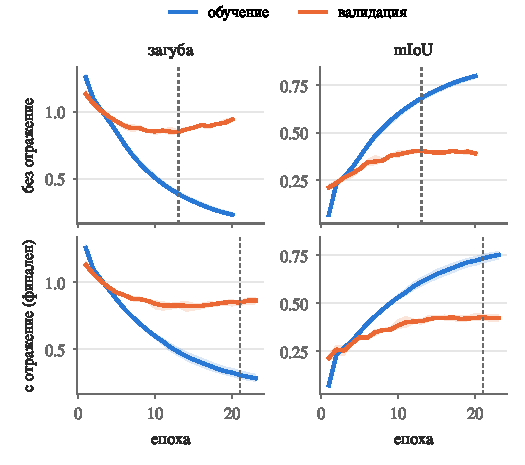
\includegraphics[width=\columnwidth]{overfitting_curves_bg.pdf}
\caption{Криви на обучение без (горе) и с (долу) отражение, средно от 3 обучения. Валидационната
загуба расте, докато загубата при обучение намалява. Пунктир: епохата с най-добър валидационен mIoU.}
\label{fig:curves}
\end{figure}

\begin{figure}[!htbp]
\centering
\begin{tikzpicture}
\definecolor{trainC}{HTML}{2A78D6}\definecolor{valC}{HTML}{EB6834}
\begin{axis}[
  ybar, bar width=10pt, width=\columnwidth, height=4.4cm,
  ymin=0, ymax=0.9, ylabel={mIoU}, ylabel style={font=\footnotesize},
  symbolic x coords={base, r1, r2, r3}, xtick=data,
  xticklabels={FiLM\\разлика 0.35, R1\\разлика 0.32, \textbf{R2 (финален)}\\разлика 0.28, R3\\разлика 0.29},
  x tick label style={font=\footnotesize, align=center},
  y tick label style={font=\footnotesize, /pgf/number format/fixed},
  enlarge x limits=0.16,
  legend style={at={(0.5,1.02)}, anchor=south, font=\footnotesize, draw=none, fill=none, legend columns=2},
  legend cell align=left,
  nodes near coords, nodes near coords style={font=\tiny, /pgf/number format/fixed, /pgf/number format/precision=2},
  ymajorgrids, grid style={gray!25}]
\addplot[fill=trainC, draw=trainC!70!black] coordinates {(base,0.760) (r1,0.746) (r2,0.710) (r3,0.725)};
\addplot[fill=valC, draw=valC!70!black] coordinates {(base,0.413) (r1,0.424) (r2,0.432) (r3,0.433)};
\legend{обучаващи изобр., валидационни изобр.}
\end{axis}
\end{tikzpicture}
\caption{mIoU върху обучаващите и валидационните изображения за вариантите с регуляризация (избраните
чекпойнти, режим на оценяване, средно от 3 обучения). Разликата под всяка двойка измерва
преобучението.}
\label{fig:gap}
\end{figure}

\subsection{Сравнение с CLIPSeg}

Като цяло финалният модел и CLIPSeg са наравно (0.393 срещу 0.385; разликата е по-малка от
разликите между отделните обучения). Двата модела използват едни и същи замразени CLIP енкодери и
декодер с подобен размер (1.05\,M срещу 1.13\,M параметъра), така че сравнението отразява главно
обучаващите данни: по-малко от 4\,000 изречения от RefCOCO-M тук срещу много по-големия набор
PhraseCut за CLIPSeg. Разбивката по тип изречение на \cref{fig:breakdown} показва, че
двата модела са силни в различни неща. Предложеният декодер, обучен върху изречения в стила на
RefCOCO, е значително по-добър при пространствени указания (0.386 срещу 0.307). CLIPSeg, обучен
върху по-големия набор PhraseCut, е значително по-добър при изречения, които назовават обект или
негови атрибути без положение (0.530 срещу 0.407). Предложеният модел е и по-бърз: около 5.5\,ms за
изображение и изречение, от които 4.7\,ms за CLIP и 0.8\,ms за декодера, срещу 7.7\,ms за
CLIPSeg.

\begin{figure}[!htbp]
\centering
\begin{tikzpicture}
\begin{axis}[
  ybar, bar width=12pt, width=\columnwidth, height=4.6cm,
  ymin=0, ymax=0.6, ylabel={mIoU (тест)}, ylabel style={font=\footnotesize},
  symbolic x coords={m0, film, final, clipseg},
  xtick=data, xticklabels={M0 само изобр., M1 FiLM, Финален (R2), CLIPSeg},
  x tick label style={font=\footnotesize},
  y tick label style={font=\footnotesize, /pgf/number format/fixed},
  enlarge x limits=0.16,
  legend style={at={(0.02,0.98)}, anchor=north west, font=\footnotesize, draw=none, fill=none},
  legend cell align=left,
  nodes near coords, nodes near coords style={font=\tiny, /pgf/number format/fixed, /pgf/number format/precision=2},
  ymajorgrids, grid style={gray!25}]
\addplot[fill=blue!55, draw=blue!70!black] coordinates
  {(m0,0.253) (film,0.375) (final,0.386) (clipseg,0.307)};
\addplot[fill=orange!60, draw=orange!70!black] coordinates
  {(m0,0.333) (film,0.375) (final,0.407) (clipseg,0.530)};
\legend{пространствени изречения (512), други изречения (277)}
\end{axis}
\end{tikzpicture}
\caption{mIoU върху тестовото множество по тип изречение. Пространствените изречения съдържат думи
като \en{left}, \en{right} или \en{behind}.}
\label{fig:breakdown}
\end{figure}

% Wide figure defined here so that it lands at the top of the page with the 3D section.
\begin{figure*}[t]
\centering
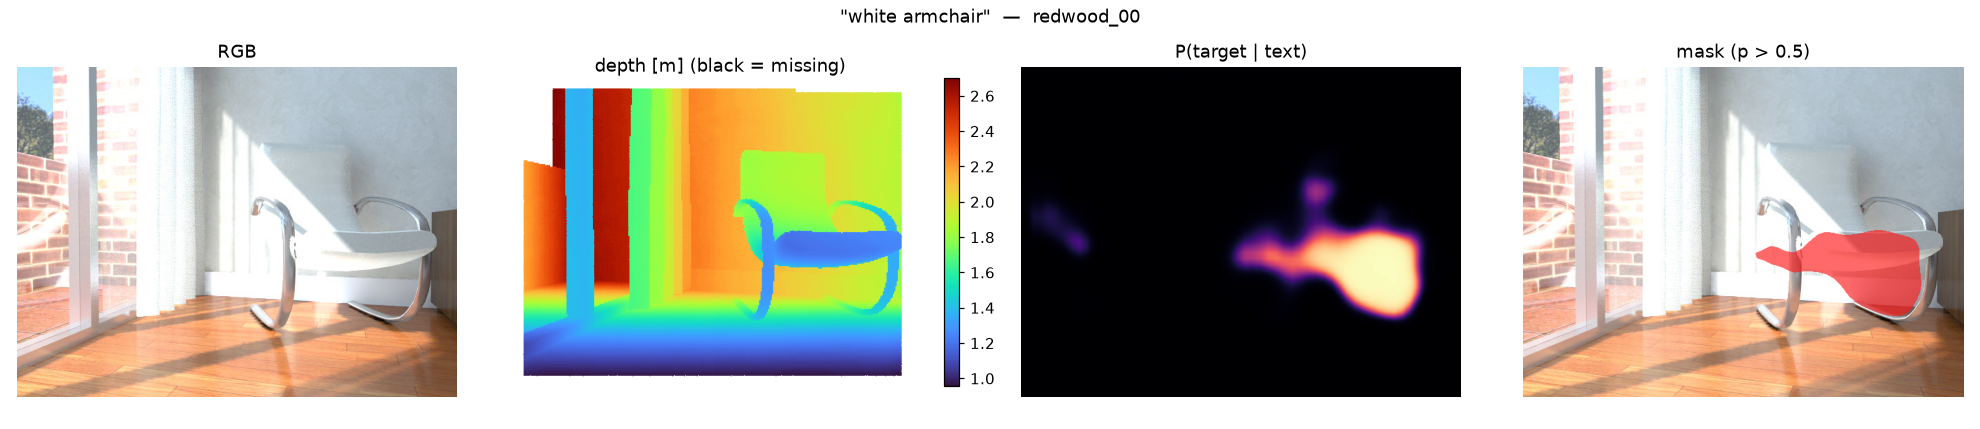
\includegraphics[width=0.95\textwidth, trim=0 0 0 30, clip]{white-armchair_redwood_00_2d.png}
\caption{\en{white armchair} върху кадър 0 от Redwood: RGB изображение, измерена дълбочина,
предсказана карта на вероятностите и маска след прагуване. Маската покрива главно седалката;
тънката метална рамка е пропусната.}
\label{fig:redwood2d}
\end{figure*}

\subsection{Неуспешни случаи}

Най-трудни са изреченията, които зависят от цвят или облекло (\en{girl in pink},
\en{man in white shirt}): 0.320 mIoU срещу 0.419 за останалите, което съответства на
предимството на CLIPSeg при атрибутите. Трудни са и претъпканите изображения с четири или повече
анотирани обекта (0.233 mIoU), най-вече защото моделът избира правилния вид обект, но грешния
екземпляр. Накрая, декодерът предсказва при $56\times56$, поради което тънките структури и точните
граници се губят.

\subsection{Локализация в 3D}

\Cref{fig:redwood2d,fig:redwood3d} показват геометричния модул върху поредицата Redwood за
изречението \en{white armchair}. Предсказаната маска се пренася от всеки от петте кадъра в общата
световна система. Тъй като креслото е неподвижно, центърът му трябва да попада в една и съща точка
от всяка гледна точка; измереното разсейване е средно 3.0\,cm и най-много 4.4\,cm (4.4\,cm и
5.2\,cm без аугментация с отражение). Петте облака от точки на сцената съвпадат без видими двойни
контури, така че оставащото разсейване се дължи на това, че маските покриват малко различни части
от креслото, а не на грешки в позите.

\begin{figure}[!htbp]
\centering
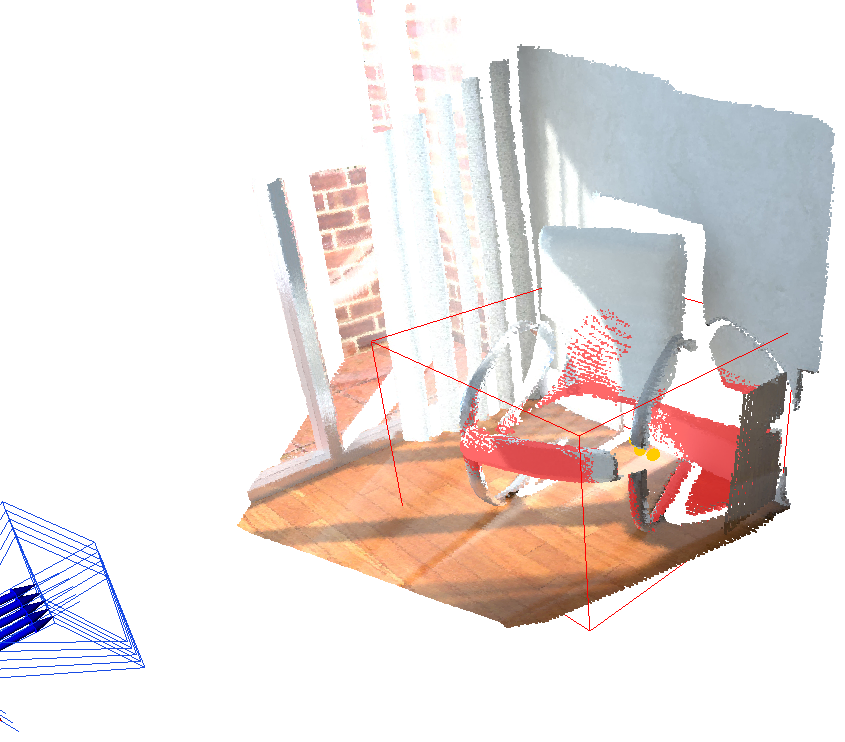
\includegraphics[width=0.85\columnwidth]{white-armchair_3d_crop.png}
\caption{Облак от точки в световни координати, обединен от пет RGB-D кадъра. Червено: точки на
обекта; жълто: центрове за всеки кадър; червена кутия: обща обхващаща кутия; синьо: пирамиди на
видимост на камерите.}
\label{fig:redwood3d}
\end{figure}

3D резултатите показват и ограниченията на 2D модела. Redwood е синтетично рендерирана сцена и се
различава от снимките в COCO, затова маската покрива главно възглавницата на седалката, а
обхващащата кутия подценява височината на креслото. Изречения за фонови области (\en{the window},
\en{the floor}) не успяват: RefCOCO анотира само отделни обекти, така че моделът е научил, че
отговорът винаги е обект, и избира най-открояващия се.

% ---------------------------------------------------------------------------
\section{\bgsc{О}{граничения и бъдещи насоки}}
\label{sec:limitations}

Основното ограничение е количеството обучаващи данни. RefCOCO-M съдържа прецизни маски за
\emph{валидационните} изображения на RefCOCO, а 833 обучаващи изображения оставят разлика от 0.28
между mIoU при обучение и валидация дори с аугментация. Обучението върху оригиналното обучаващо
множество на RefCOCO (около 17\,000 изображения, без припокриване с използваните тук) е естествената
следваща стъпка. Отчетените стойности са върху собствено разделяне на данните и не са сравними с
публикуваните резултати за RefCOCO. Възможно е също CLIP и CLIPSeg да са виждали изображения от COCO
по време на предварителното си обучение. В геометричната част всеки кадър вижда само видимите
повърхности, обхващащата кутия е успоредна на осите, а не ориентирана, а 3D резултатът е
локализация, а не план за хващане или манипулация. Декодиране с по-висока разделителна способност,
ориентирани кутии и обединяване на маските от отделните кадри в обща обемна карта са естествени
разширения.

% ---------------------------------------------------------------------------
\section{\bgsc{З}{аключение}}
\label{sec:conclusion}

Декодер с около един милион параметъра върху замразени CLIP признаци може да свързва референтни
изрази с обекти: обуславянето по текст чрез FiLM подобрява mIoU върху тестовото множество от 0.281 на
0.393, достига предварително обучения модел CLIPSeg като цяло и ясно го превъзхожда при
пространствени указания. Хоризонталното отражение, съобразено с езика, при което \en{left} и
\en{right} се разменят, е евтин и ефективен регуляризатор за тази задача. В съчетание с модела на
камера с точков отвор и калибрирана RGB-D камера 2D маските се превръщат в съгласувана 3D
локализация с точност от няколко сантиметра между различни гледни точки. Това е първа стъпка от
\enquote{какво каза потребителят} към \enquote{къде трябва да погледне роботът}.

\section*{\bgsc{П}{рограмен код}}

Кодът, разделянето на данните и скриптовете за всички резултати:
\url{https://github.com/Apsie09/Text-Guided-Segmentation-3D}.

\bibliographystyle{IEEEtran}
\bibliography{refs}

\end{document}
